%%%%%%%%%%%%%%%%%%%%%%%%%%%%%%%%%%%%%%%%%%%%%%%%%%%%%%%%%%%%%%%%%%%%%%%%%%%%%%%%
\chapter{Challenges of Kernel Space}
%%%%%%%%%%%%%%%%%%%%%%%%%%%%%%%%%%%%%%%%%%%%%%%%%%%%%%%%%%%%%%%%%%%%%%%%%%%%%%%%
\label{sec:challenges}

\revision{In this chapter, we discuss several problems that stand in the way of systematic exploration's applicability to kernel space. We address these problems in part with certain aspects of Landslide's design and in part by relying on the user to provide important information, which we discuss in Chapter~\ref{sec:design} and Chapter~\ref{sec:using} respectively.}

\section{Causes of Concurrency}

In user space, a systematic exploration tool may cooperate with the underlying kernel to help control the concurrent behaviour of the system\cite{dbug-ssv}. Simple system call invocations can cause a particular thread to run at a particular time, or to block while another thread runs first.

In kernel space, however, the scheduler is part of the system being tested, and we can no longer always interrupt the execution of a test case to ask the scheduler to instantly start running a different thread.
\begin{itemize}
	\item {\bf Non-preemptibility.} Certain regions of code may be non-preemptible, so a testing tool must know when it is legal to preempt a kernel thread.
	\item {\bf The context switcher.} A context switch between threads is no longer ``instantaneous'': many instructions must be run between when we decide to preempt and when the next thread begins running, and the tool must be aware of this ``intermediate state''. A tool must be aware of the context switch process both to avoid flooding the kernel with interrupt frames that would overflow the stack, and to be able to ignore shared memory conflicts inherent to all thread transitions (Section~\ref{sec:por-independence}).
	\item {\bf Run-queue tracking.} The kernel's scheduler and the tool must cooperate in some way so that the tool can both know what threads are runnable at every point during execution and cause any given runnable thread to begin running in place of the current one.
\end{itemize}

\begin{figure*}[t]
	\begin{center}
	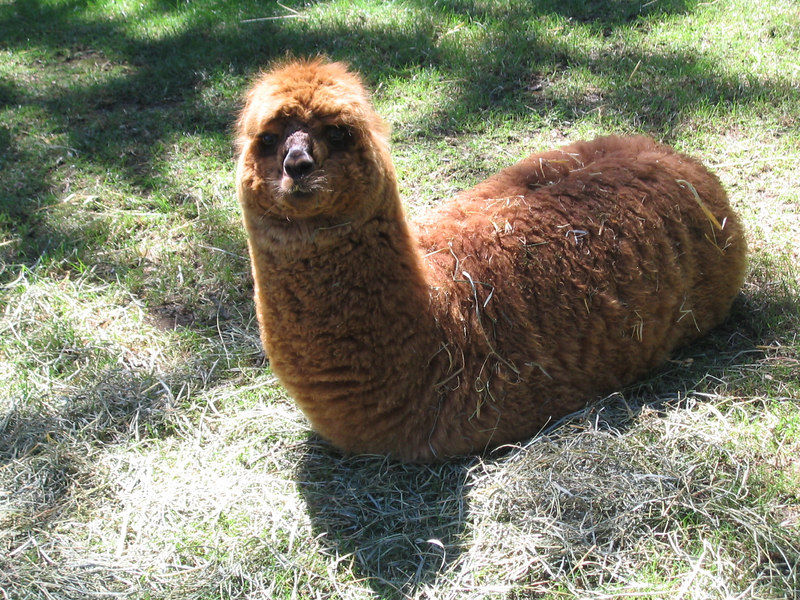
\includegraphics[width=0.65\textwidth]{vip1066720.jpg}
	\end{center}
	\caption{{\em !`Cuidado! !`Las llamas son muy peligrosas!}\cite{de0u}}
\end{figure*}

\section{Ad-hoc Thread Communication}

Inter-thread communication can be much more ad-hoc in kernel-space than in user-space\hspace{0in}\cite{datacollider}, and a systematic testing framework needs to be aware of all the kernel's synchronisation idioms.

\begin{itemize}
	\item {\bf Avoiding reliance on message-passing.} Some systems for user-space systematic testing require that threads communicate only by message-passing, to better track the concurrency relationships between thread transitions\cite{dbug-ssv}. With few exceptions\cite{barrelfish}, kernels do not rely on message-passing as a primary communication mechanism, and to be compatible with the kernels of today, a testing framework must allow for less idealised state-sharing (Section~\ref{sec:components-memory}).
	\item {\bf Recognising blocked threads.} It is difficult to detect when threads are ready to do useful work. Even if notionally runnable, they may be waiting in a yield loop (Sections~\ref{sec:using-annotations} and \ref{sec:future-linux}), which can be difficult to discern without an understanding of whatever shared resource the thread is waiting for. A tool that did not recognise this might decide to attempt to run that thread over and over, and get stuck because the other threads would never be allowed to make progress.
	\item {\bf Thread lifecycle tracking.} It is also difficult to demarcate threads' lifecycles: when a new thread gets created, when is it available to run? When a thread is exiting, at what point does it stop running code (Section~\ref{sec:using-annotations})? In user-space, these boundaries are defined by the system call instructions, but in kernel-space, the boundary is fuzzier.
	\item {\bf Use of virtual memory.} The kernel's complete control over the machine's virtual memory system means a system for tracking memory accesses must be aware of changing virtual memory mappings (Section~\ref{sec:using-requirements}). A tool not aware of virtual memory might falsely identify whether or not two transitions' memory accesses conflict.
\end{itemize}

\section{Kernel Design Independence}
\label{sec:challenges-design}

One challenge particular to the context of 15-410 is that the kernels Landslide must be able to test may all use slightly different implementations to achieve the same goals.
\revision{While 15-410's kernel project mandates that students implement the Pebbles specification, students are free to make their own design decisions under the hood, which can result in significantly different scheduler behaviour among multiple kernels. In general, Landslide may rely on concrete details provided by kernel specifications, but must be compatible with arbitrary implementation details.}
For Landslide to be generally applicable to many different kernels, even only multiple ones that implement the same specification (such as Pebbles), it must make some abstract assumptions about the kernel design which are compatible with many different implementations.

% In certain avenues of future work (Section~\ref{sec:future-linux}), remaining agnostic of most implementation details becomes less of an issue. For example, if we target Landslide to Linux, it is unlikely that core scheduler or interrupt-handling behaviour will change for as long as Landslide remains useful for finding bugs. In 15-410, however, repeated re-targetting is a necessity.

We built Landslide to be compatible with multiple designs for the following major scheduling behaviours:

\begin{itemize}
	\item {\bf Runqueues}: Does the kernel store the currently-running thread on the runqueue, or is it ``checked out'' while running and stored separately?
	\item {\bf Mutexes}: When a thread blocks on a mutex, is it left on the runqueue in a yield loop, or is it explicitly descheduled (e.g., moved from the runqueue to another queue)? In yield-looping mutexes, when do blocked threads become ``unblocked'', notionally? (This might happen before the blocked thread runs next.)
	\item {\bf Idling}: Does the kernel have an explicit idle thread, or is there an idle loop that runs on the stack of whatever thread was last running? Do explicit idle threads run their idle loop in userspace or in kernelspace?
	\item {\bf Thread Creation}: When a thread is newly forked, is it placed onto the runqueue for later, or is it context-switched to immediately? Do just-forked threads begin life through the usual context-switch-return path, or is there a special path for that?
	\item {\bf Test Lifecycle}: Apart from running on a particular input that the user wishes to test, the kernel may need to perform extra work, such as initialisation (e.g., the bootup process) and housekeeping (e.g., cleaning up dead processes).
	\revision{Though the entire kernel is notionally the system under test, the user-space test case expresses what the user is actually interested in, and some of this extra work is irrelevant.}
	Which parts of this work should be included in or excluded from the test?
\end{itemize}
